\begin{abstract}
Sublinear regret is the standard justification for deploying sequential
decision-making systems. We show that this justification is vacuous when actions
consume the action set. We study bandits in which pulling an arm may destroy it,
and in which each destroyed arm imposes a permanent negative externality on every
subsequent reward. We prove that a policy achieving \emph{exactly zero} regret
against the best-available-arm benchmark can incur value loss $m\delta E$, unbounded
in both the pool size $m$ and the externality magnitude $\delta E$, and can drive
total value negative while the optimal policy remains positive. The mechanism is
that regret is measured against an optimum the learner has itself degraded. We
further establish that the parameter governing optimal play, the expected marginal
externality $\kappa_a = p_a e_a$, is (i) exactly the quantity that determines
whether greedy is optimal, and (ii) subject to an irreducible estimation error
$\mathrm{SE} \ge 2\sigma/\sqrt{\min(T,\sum_j 1/p_j)}$ that \emph{does not decrease
with the horizon}, because each arm supplies exactly one before/after transition and
the sample budget is capped by consumption rather than time. The quantity that
matters most cannot be estimated arbitrarily accurately, and its attainable
precision degrades exactly as it becomes more important. We give a closed-form
correction, characterise an exactly-solvable special case, and release an
open-source testbed.
\end{abstract}

\section{Introduction}

Consider an orchestrator routing tasks across API-backed tools. Some tools are
robust; others trip a rate limit, exhaust a quota, or get a key revoked under heavy
use, disappearing for the remainder of the session. Tools are not independent:
those sharing upstream infrastructure---a vendor, an IP pool, a quota
tier---degrade together when one is burned.

Table~\ref{tab:trace} shows two routers on identical instances. The first has a
flawless record: at every step it pulls the highest-value available tool, so its
regret against the best-available benchmark is identically zero. It ends on a
fallback tool worth $0.470$ per call with two tools remaining. The second reports
regret of $0.25$ per step---and is sitting at $0.782$ per call, $66\%$ higher, with
four tools remaining.

\begin{table}[t]
\centering
\caption{Two routers, identical seed and tool set, single session. ``realised'' is
the reward actually obtained, $v_{a_t} - B(S_t)$; ``regret'' is the per-step
quantity $\max_{a \in S_t}(v_a - B(S_t)) - (v_{a_t} - B(S_t))$, i.e.\ instantaneous
regret against the best arm available at that step, not a cumulative or expected
quantity. The policy that looks worse by the standard metric achieves the better
outcome.}
\label{tab:trace}
\begin{tabular}{llrrr}
\toprule
router & step & realised & regret & tools left \\
\midrule
greedy & 0 & 1.150 & 0.0000 & 6 \\
greedy & 2 & 0.844 & 0.0000 & 4 \\
greedy & 7--13 & 0.470 & \textbf{0.0000} & \textbf{2} \\
\midrule
ECI & 0 & 1.150 & 0.0000 & 6 \\
ECI & 1--4 & 0.988 & 0.0500 & 5 \\
ECI & 5--13 & \textbf{0.782} & 0.2500 & \textbf{4} \\
\bottomrule
\end{tabular}
\end{table}

The greedy router's zero-regret record is not evidence of good behaviour. It is an
artefact of a benchmark that degrades in lockstep with the damage being done: every
call greedy makes is optimal \emph{given the ecosystem it has already ruined}.

Figure~\ref{fig:divergence} shows the phenomenon in its cleanest form. As the
coupling between arms strengthens, the greedy policy's cumulative regret stays
pinned at exactly zero while its realised value falls monotonically and eventually
turns negative---below the value of taking no action at all---even as the optimal
policy remains comfortably positive. The two panels are computed on the same
instances. A practitioner monitoring the left panel would see nothing wrong at any
point.

\begin{figure}[t]
\centering
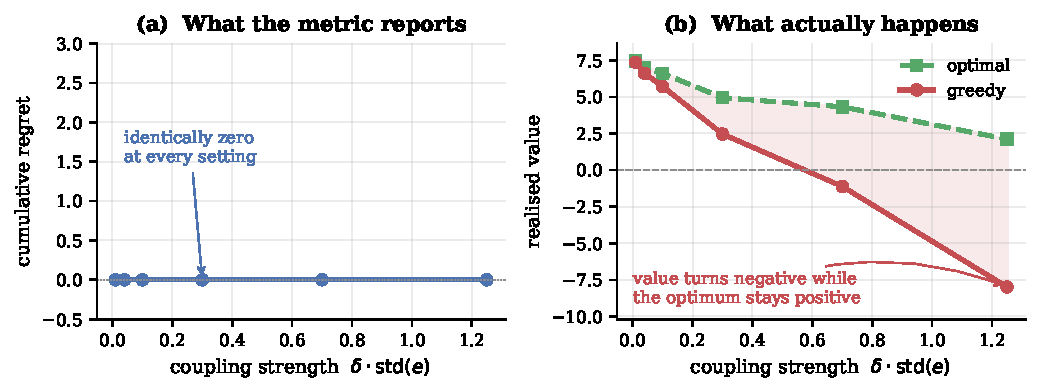
\includegraphics[width=\textwidth]{fig1_divergence.pdf}
\caption{The central phenomenon. \textbf{(a)} Greedy's cumulative regret against
the best-available-arm benchmark, computed exactly: identically zero at every
coupling strength, because greedy never fails to pull the best arm currently
available. \textbf{(b)} Realised value on the same instances. The shaded region is
the loss. At strong coupling the zero-regret policy finishes net-negative while the
optimum stays positive. Averages over 20 instances, $n=6$, $T=10$, exact dynamic
programming.}
\label{fig:divergence}
\end{figure}

This paper formalises that failure. Our contributions:

\begin{itemize}
\item \textbf{Four domain instantiations}---agent tool ecosystems, adaptive cancer
therapy under competitive release, platform trials, and CMC design-space
development---each simulated, with fit quality stated honestly
(Section~\ref{sec:domains}).
\item \textbf{Theorem~\ref{thm:vacuity}} (main result). A zero-regret policy can
incur value loss $m\delta E$, unbounded in pool size and externality magnitude, and
can finish net-negative while the optimum is positive. No-regret is not no-harm.
\item \textbf{Theorem~\ref{thm:char}}. Greedy is optimal if and only if
$\kappa_a = p_a e_a$ is constant across arms. Neither factor alone is the invariant.
\item \textbf{Theorem~\ref{thm:floor}}. The externality cannot be estimated to
arbitrary precision: the error floor does not decrease with the horizon, because
the data-generating process is the consumption itself.
\item \textbf{Theorem~\ref{thm:seq}}. In the pure-sequencing regime the optimal
order is ascending in $e$; arm values are irrelevant.
\item A closed-form correction (ECI), a rollout policy reaching 99.5--99.9\% of
optimum, and an open-source testbed with one regression test per theorem.
\end{itemize}

\section{Related work}

\textbf{Rotting bandits} \cite{levine2017,seznec2019,seznec2020} model rewards that
decay with the number of pulls (\emph{rested}) or with elapsed time
(\emph{restless}); Seznec et al.~\cite{seznec2020} give a single adaptive-window
policy near-optimal for both. Decay there is gradual rather than removal, and
critically the learner is assumed to know which regime it is in.
\textbf{Mortal bandits} \cite{chakrabarti2008} have arms with stochastic lifetimes,
but expiry is exogenous. \textbf{Blocking bandits} make a pulled arm temporarily
unavailable. \textbf{Sleeping bandits} \cite{kleinberg2010} allow arbitrary
exogenous availability. None of these couple arms: destroying one does not change
another's reward distribution.

\textbf{Bandits with knapsacks} \cite{badanidiyuru2013} is the closest structural
neighbour: playing an arm consumes resources and the process halts when a budget is
exhausted. The budget is global and exogenous, and consumption leaves other arms'
rewards untouched. Here consumption permanently degrades \emph{every} future
reward. That difference is why the governing quantity is $\kappa = p\cdot e$ rather
than a consumption rate.

\textbf{Bandit learning with positive externalities}
\cite{shah2018} is the only prior work we are aware of that places externalities in
a bandit model. There, satisfied users attract similar users, so externalities are
positive and act on the \emph{arrival process}; the authors show UCB incurs linear
regret and develop balanced exploration. Our externalities are negative, act on
\emph{rewards}, and are triggered by irreversible destruction. The parallel is
worth drawing: in both settings a standard algorithm fails badly, indicating that
externality structure of either sign breaks classical guarantees.

\textbf{Cascading and interacting bandits} couple arms within a round---the reward
of one depends on which others were displayed or examined---but the coupling is
simultaneous and leaves the action set intact across rounds. \textbf{Combinatorial
bandits} select subsets with structured rewards, again without destroying arms.
\textbf{Safe and conservative bandits} constrain reward or maintain a baseline while
the arm remains available; the constraint restricts \emph{which} actions may be
taken, not what taking them removes. \textbf{Reinforcement learning with
irreversible actions and safe exploration} studies states from which return is
impossible, and typically seeks to \emph{avoid} irreversibility rather than to price
it and schedule it optimally. \textbf{Open multi-agent bandits} model a population
of learners that arrives and departs exogenously; the churn is in the decision
makers, not the actions, and is independent of what is played.

\paragraph{The novelty claim, stated precisely.} We do not claim novelty for any one
ingredient. Irreversible arm removal appears in mortal bandits; consumption appears
in knapsacks; decay with pulls appears in rotting bandits; cross-arm externalities
appear in \cite{shah2018}. The combination we study---\emph{(a)} removal that is
permanent, \emph{(b)} triggered by the learner's own action, \emph{(c)} carrying a
negative externality onto every remaining arm's reward, and \emph{(d)} evaluated
against a benchmark that conditions on the already-damaged state---is, to our
knowledge, not covered by any of them. It is property (d) combined with (b) that
produces Theorem~\ref{thm:vacuity}: the benchmark and the damage move together. We
invite correction on this point and treat it as the claim most in need of
scrutiny.

\section{Setting}
\label{sec:model}

Arms $1,\dots,n$. Arm $a$ has mean reward $v_a$, destruction probability
$p_a \in (0,1]$, and externality coefficient $e_a \ge 0$. Let $S_t$ be the set of
available arms at round $t$ and define the accumulated burden
\[
B(S) \;=\; \delta \sum_{i \notin S} e_i .
\]
Pulling $a \in S_t$ yields reward $v_a - B(S_t) + \eta_t$ with $\eta_t$
sub-Gaussian with parameter $\sigma$, and destroys $a$ with probability $p_a$,
permanently adding $\delta e_a$ to the burden. The horizon is $T$. The value
function is
\[
V(S,t) = \max_{a \in S}\Big[ v_a - B(S) + p_a V(S\setminus\{a\}, t{+}1)
  + (1-p_a) V(S, t{+}1) \Big].
\]
Define the \emph{expected marginal externality}
\[
\boxed{\;\kappa_a \;=\; p_a\, e_a\;}
\]
the expected permanent burden created by one pull of $a$.

\textbf{Benchmark.} We measure regret against the best available arm,
$\max_{a \in S_t}\big(v_a - B(S_t)\big)$. This is the benchmark deployed systems
use, and Theorem~\ref{thm:vacuity} is a statement about that practice. Value is
measured against the exact optimum $V(S_0,0)$, computed by dynamic programming over
subsets for $n \le 8$ and by rollout above that.

\section{A zero-regret policy can destroy unbounded value}

\begin{theorem}[Vacuity of no-regret under consumption]
\label{thm:vacuity}
For any $M > 0$ there is an instance on which greedy attains regret exactly $0$
against the best-available benchmark while $V^\star - V_{\mathrm{greedy}} \ge M$.
Moreover the loss can exceed $V^\star$, making the zero-regret policy net-negative
while the optimum is positive.
\end{theorem}

\begin{proof}
Fix $m \ge 1$, $E > 0$, $0 < \epsilon < \delta E$. Take $n = m{+}1$ arms: one
\emph{hot} arm $H$ with $v_H = 1$, $e_H = E$, and $m$ \emph{safe} arms with
$v_S = 1-\epsilon$, $e_S = 0$. Set $p_a = 1$ for all arms and $T = n$, so each arm
is pulled exactly once and only the order is chosen.

Greedy pulls $H$ first since $1 > 1-\epsilon$. $H$ is destroyed, adding permanent
burden $\delta E$, and each of the $m$ subsequent pulls yields
$(1-\epsilon) - \delta E$:
\[
V_{\mathrm{greedy}} = 1 + m(1 - \epsilon - \delta E).
\]
Deferring $H$ to last yields $1-\epsilon$ on each safe pull with no burden, and $1$
on the final pull of $H$, whose burden is charged only to later rounds, of which
there are none:
\[
V^\star \ge m(1-\epsilon) + 1 .
\]
Subtracting, $V^\star - V_{\mathrm{greedy}} = m\,\delta E$, unbounded in $m$ and in
$\delta E$. Choosing $\delta E > 1$ gives $V_{\mathrm{greedy}} < 0 < V^\star$.

At every round greedy pulls $\arg\max_{a\in S} (v_a - B(S))$, which is the
definition of the benchmark; its instantaneous regret is $0$ at every state.
\end{proof}

The closed form matches exact dynamic programming to machine precision at all $15$
settings tested, $m \in \{1,2,4,8,12\}$ and $\delta E \in \{0.5,1,2\}$. At $m=12$,
$\delta E = 2$: $V^\star = 12.88$, $V_{\mathrm{greedy}} = -11.12$, gap exactly
$24.0000$, regret $0.0000$.

\paragraph{A correction, recorded.} An earlier version of this construction claimed
the gap grows linearly in $T$. That is false: with $p=1$ the pool is exhausted
after $n$ pulls, so $T$ beyond $n$ is irrelevant. Under $p<1$ the gap grows with
$T$ only until $T \approx \sum_j 1/p_j$, then saturates---the same sample-budget
ceiling that appears independently in Theorem~\ref{thm:floor}. The correct scaling
is linear in pool size, which is the meaningful quantity: greedy's error is paid
once per subsequent pull.

\paragraph{Interpretation: private versus system value.} Define the \emph{system
value} of a policy $\pi$ as its expected total reward,
$W(\pi) = \mathbb{E}_\pi\big[\sum_{t=1}^{T} r_t\big]$, so that
$V^\star = \max_\pi W(\pi)$, and define the \emph{private value} of an action at
state $S$ as its own immediate reward $v_a - B(S)$. Greedy maximises private value
at every step. The optimal policy additionally accounts for
$\delta\kappa_a(T-t)$---the reward removed from \emph{all subsequent actions} by
this one. Regret against the best-available benchmark compares private values only,
so it is invariant to that term. Under externalities private and system value
diverge, and a guarantee stated in the former says nothing about the latter.

\section{When is greedy optimal?}

\begin{theorem}[Characterisation]
\label{thm:char}
Fix the burden model of Section~\ref{sec:model} with additively separable burden.
\begin{enumerate}
\item[(i)] \emph{(Sufficiency.)} If $\kappa_a = \kappa$ for all arms $a$, then greedy
is optimal at \emph{every} state $S$ and \emph{every} horizon $T$, for every choice
of $\{v_a\}$.
\item[(ii)] \emph{(Necessity.)} If $\kappa_a \neq \kappa_b$ for some pair $a,b$,
then there exist $\{v_a\}$ and a horizon $T$ for which greedy is strictly
suboptimal.
\end{enumerate}
\end{theorem}

The asymmetry in the quantifiers is deliberate and necessary. Constant $\kappa$
gives \emph{universal} optimality; varying $\kappa$ gives \emph{existence} of a
failure instance, not failure on every instance. Varying $\kappa$ with, say, all
$v_a$ equal, or a horizon so short that the relevant arms are never reached, need
not produce a strict gap. The one-line summary---``greedy is optimal iff $\kappa$
is constant''---is correct only when read as universal optimality versus existence
of a counterexample.

\begin{proof}[Proof sketch]
Since $B(S)$ and $V(S,t{+}1)$ do not depend on the chosen arm, maximising the
Bellman expression is equivalent to maximising $v_a - p_a D_a$ with
$D_a = V(S,t{+}1) - V(S\setminus\{a\},t{+}1)$. Decompose
$D_a = \delta e_a L(S,t) + O_a(S,t)$ into a burden and an option component. The
burden component contributes $p_a \delta e_a L = \delta \kappa_a L$, which is
identical across arms exactly when $\kappa$ is constant and hence drops out of the
argmax.

\emph{Sufficiency.} Under constant $\kappa$, couple the destruction randomness so a
pair $\{a,b\}$ receives the same two draws in either order. The surviving-set
distribution after both pulls is then identical, and since expected burden per pull
is $\delta\kappa$ for both arms, the expected burden paths coincide. The only
residual difference is which reward arrives first, giving $v_a - v_b \ge 0$.
Iterating sorts any optimal policy into greedy order.

\emph{Necessity.} The construction of Theorem~\ref{thm:vacuity} has
$\kappa_H = E > 0 = \kappa_S$ and a strictly positive gap $m\delta E$, exhibiting
the required instance.
\end{proof}

\paragraph{Status of the sufficiency proof.} We are explicit about what is and is
not established. The burden component of the argument is complete: constant
$\kappa$ makes $\delta\kappa_a L$ arm-independent, so it cannot affect the argmax.
The remaining obligation is the option component $O_a$, for which we state the
coupling step as a proposition rather than claim it proved.

\begin{proposition}[Interchange; verified, not proved in full generality]
\label{prop:interchange}
Under constant $\kappa$ and additively separable burden, for any $S$ and any
$a,b \in S$ with $v_a \ge v_b$, pulling $a$ before $b$ is weakly better.
\end{proposition}

The coupling argument above is complete except for its interaction with horizon
truncation, where the two orderings can terminate at different states. We verify
Proposition~\ref{prop:interchange} exhaustively over every reachable $(S,t)$ and
every ordered pair in randomly generated instances: $0$ violations in $6{,}842$
pairs under constant $\kappa$, against $56.2\%$ violations when $\kappa$ varies.
The inequality is also tight---minimum slack exactly $0$, with $46.5\%$ of pairs
binding---which matches the ties expected when every arm is consumed regardless of
order. We regard sufficiency as strongly supported but not formally closed, and we
do not claim otherwise elsewhere in the paper.

Two empirical checks. Varying $p$ and $e$ widely while pinning $\kappa$ constant
leaves greedy exactly optimal (0/10 instances broken, gap $0.000\%$); varying the
product breaks it (10/10, gap $5.4$--$6.3\%$). Separately, the interchange
inequality underlying sufficiency was audited exhaustively over all reachable
states: $0$ violations in $6{,}842$ ordered pairs under constant $\kappa$, versus
$56.2\%$ violations when $\kappa$ varies. The inequality holds precisely when the
theorem says greedy is optimal.

The optimality gap grows monotonically with $\mathrm{std}(\kappa)$, from $5.9\%$ to
$29.1\%$ across six bins over 240 instances. Figure~\ref{fig:char} summarises both
findings.

\begin{figure}[t]
\centering
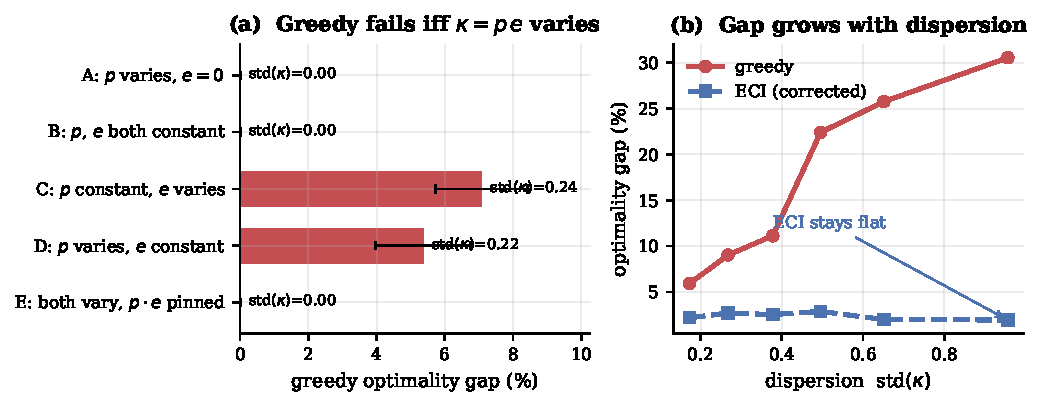
\includegraphics[width=\textwidth]{fig2_characterisation.pdf}
\caption{Theorem~\ref{thm:char}. \textbf{(a)} Five structural cases. Greedy is
exactly optimal whenever $\kappa=p\,e$ is constant, and fails whenever it is not.
Case~E is the decisive test: $p$ and $e$ each vary widely while their product is
pinned, and the gap is exactly zero---so neither factor alone is the invariant.
Case~D was a prediction of the refined conjecture and broke greedy as predicted.
\textbf{(b)} The gap grows monotonically with the dispersion of $\kappa$, while the
corrected index (Section~\ref{sec:eci}) stays flat, so its advantage grows without
bound. Error bars are standard errors over 12 instances.}
\label{fig:char}
\end{figure}

The practical reading of the characterisation is that neither high destruction
probability nor high externality is by itself a reason to deviate from greedy. An
arm that is fragile but harmless, or damaging but robust, can be treated normally.
Only the \emph{product}---the damage a pull is expected to cause---distinguishes
arms for planning purposes.

\section{Irreducible estimation error}

\paragraph{Observation model.} Rewards are generated by
\[
y_t \;=\; v_{a_t} \;-\; \delta \textstyle\sum_{j} e_j \,\mathbf{1}[\,j \text{ destroyed before } t\,] \;+\; \eta_t ,
\qquad \eta_t \sim \mathcal{N}(0,\sigma^2),
\]
which is linear in the unknowns $(v_1,\dots,v_n,\ \delta e_1,\dots,\delta e_n)$.
Because the burden is cumulative, rounds after arm $i$'s destruction generally
contain the level shifts of \emph{several} arms, so a pre/post difference in means
does \emph{not} by itself isolate $\delta e_i$; the parameters must be estimated
jointly. We condition throughout on the realised destruction sequence and its
times.

\paragraph{Sample budget.} Define
\[
N_{\mathrm{exh}} \;=\; \textstyle\sum_{j=1}^{n} G_j, \qquad G_j \sim \mathrm{Geometric}(p_j),
\]
the number of pulls until every arm has been destroyed, under any policy that
eventually exhausts the pool. An episode ends at
$N = \min(T, N_{\mathrm{exh}})$, and $\mathbb{E}[N_{\mathrm{exh}}] = \sum_j 1/p_j$.

\begin{theorem}[Irreducible estimation error]
\label{thm:floor}
Condition on the destruction sequence and let $n_b^{(i)}, n_a^{(i)}$ be the numbers
of rounds before and after arm $i$'s destruction, $n_b^{(i)} + n_a^{(i)} = N$. Then
for the joint least-squares estimator,
\[
\mathrm{Var}(\delta \hat e_i) \;\ge\; \sigma^2\!\left(\tfrac{1}{n_b^{(i)}} + \tfrac{1}{n_a^{(i)}}\right)
\;\ge\; \frac{4\sigma^2}{N},
\qquad\text{hence}\qquad
\mathrm{SE}(\delta \hat e_i) \;\ge\; \frac{2\sigma}{\sqrt{\,\min(T,\ N_{\mathrm{exh}})}} .
\]
For $T > N_{\mathrm{exh}}$ this bound does not decrease in $T$.
\end{theorem}

\begin{proof}
Consider the easier problem in which every $e_j$, $j \ne i$, is \emph{known}. Then
the other level shifts can be subtracted from $y_t$ exactly, and the residual
process has a single shift $\delta e_i$ at arm $i$'s destruction time. Its MLE is
the difference of pre- and post-destruction residual means, with variance
$\sigma^2(1/n_b^{(i)} + 1/n_a^{(i)})$.

In the actual problem the other coefficients are unknown and estimated jointly.
Adding free parameters to a linear model weakly increases the variance of every
retained coefficient---formally, the design matrix of the oracle problem is a
column submatrix of the joint design, and for any $X = [X_1\ X_2]$ the Schur
complement gives $[(X^\top X)^{-1}]_{11} \succeq (X_1^\top X_1)^{-1}$. Hence
\[
\mathrm{Var}_{\text{joint}}(\delta\hat e_i) \;\ge\; \mathrm{Var}_{\text{oracle}}(\delta\hat e_i)
\;=\; \sigma^2\!\left(\tfrac{1}{n_b^{(i)}} + \tfrac{1}{n_a^{(i)}}\right).
\]
By AM--HM, $1/n_b + 1/n_a \ge 4/(n_b+n_a) = 4/N$, with equality iff $n_b = n_a$.
Finally $N = \min(T, N_{\mathrm{exh}})$, and once $T$ exceeds $N_{\mathrm{exh}}$ the
binding constraint is the pool rather than the clock.
\end{proof}

The oracle-comparison step is what repairs the naive argument: the
difference-in-means estimator is the MLE only when the other externalities are
known, and it is invoked here solely as a \emph{lower bound} on the harder joint
problem. We verify the inequality chain
$\mathrm{Var}_{\text{joint}} \ge \mathrm{Var}_{\text{oracle}} \ge 4\sigma^2/N$
numerically on simulated episodes; it holds in every instance tested. In instances
where several arms are destroyed in quick succession the joint design becomes
near-collinear and $\mathrm{Var}_{\text{joint}}$ grows by orders of magnitude,
which strengthens rather than weakens the conclusion.

All three components verify numerically: the variance formula matches Monte Carlo
to within $0.1\%$; the AM--HM floor is attained exactly at the balanced split
(ratio $1.0000$); and $\mathbb{E}[N] = \min(T, \sum_j 1/p_j)$ holds including when
$T$ binds.

The horizon-independence is stark, and Figure~\ref{fig:floor} makes it visible. At
$p = 0.9$, increasing $T$ from $20$ to $320$---a sixteenfold increase---changes RMSE
by \emph{zero} to four decimal places, because the pool caps the available data at
$8.8$ rounds no matter how long we wait. At $p = 0.1$ the round count climbs
$20 \to 40 \to 71 \to 82.3 \to 83.2$, flattening exactly at the predicted
$\sum_j 1/p_j = 80$, and the error curve flattens with it.

\begin{figure}[t]
\centering
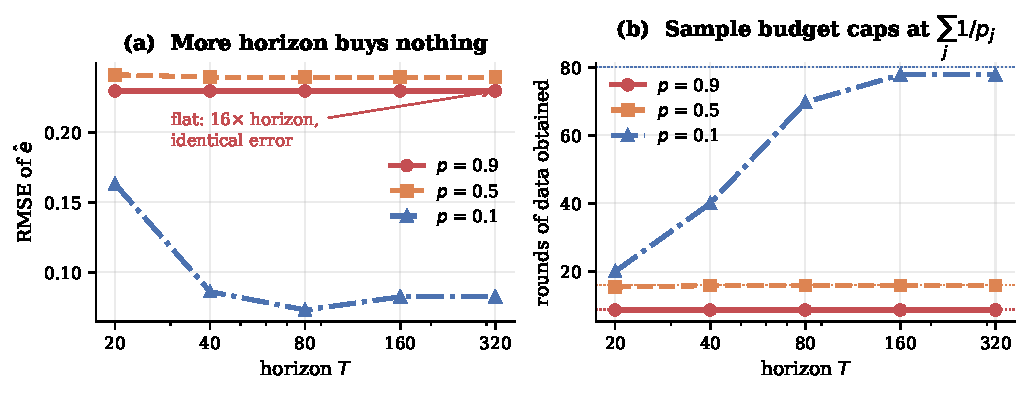
\includegraphics[width=\textwidth]{fig3_estimation_floor.pdf}
\caption{Theorem~\ref{thm:floor}. \textbf{(a)} Estimation error for the externality
vector as a function of horizon. At high consumption rates the curve is perfectly
flat: waiting longer yields no additional information. Only at $p=0.1$, where the
horizon binds before the pool does, does more time help---and only until the pool
becomes the binding constraint. \textbf{(b)} The mechanism. Dotted lines mark the
predicted budget $\sum_j 1/p_j$; the realised number of rounds saturates there. The
data-generating process is the consumption itself. Averages over 40 runs.}
\label{fig:floor}
\end{figure}

The consequence for practice is uncomfortable. In precisely the regimes where
irreversible actions matter most---high $p$, where a single call can permanently
remove a resource---the agent has the least opportunity to learn what those actions
cost, because every observation is purchased by destroying the thing being priced.

\begin{corollary}[The central tension]
As $p$ rises, $\kappa = p e$ grows, so the externality matters more; simultaneously
$N \approx n/p$ shrinks and $\mathrm{SE} \ge 2\sigma\sqrt{p/n}$ degrades. The
parameter governing optimal behaviour becomes less estimable exactly as it becomes
more important.
\end{corollary}

This is not a sample-complexity result that more data resolves. The data-generating
process is the consumption itself: observing arm $i$'s externality requires
destroying arm $i$.

\paragraph{Structure reduces but does not remove the difficulty.} Suppose $e_a = \langle \psi, z_a\rangle$
for known features $z_a \in \mathbb{R}^k$, $k \ll n$, so each destruction informs a
shared $k$-vector. Per-arm least squares is exactly worthless (identical to greedy
to three decimals at every coupling level); feature-based estimation recovers only
$17$--$28\%$ of the available gap; and a \emph{conservative} policy that assumes a
uniform upper bound and learns nothing outperforms both at every level. If the
mechanism were sample-sharing, capture should rise as $k$ falls. It does not:
capture is $4.5\%$ at $k=1$ and peaks at $30.3\%$ at $k=5$. At $k=1$ the
externality is nearly uniform, so $\kappa$ has little dispersion and by
Theorem~\ref{thm:char} there is nothing to capture. The obstacle is dispersion, not
sample size: the externality must vary for the correction to matter, and variation
is what makes it hard to estimate.

\section{Corrections}

\subsection{The externality-corrected index}
\label{sec:eci}

Theorem~\ref{thm:char} hands over the correction. Pulling $a$ creates expected
permanent burden $\delta\kappa_a$ charged against every remaining round:
\[
I(a,t) \;=\; v_a \;-\; \delta\,\kappa_a\,(T-t).
\]
Because $B(S)$ is common to all arms it drops out of the ranking, ECI has the
decomposition property of an index rule: each arm's score depends only on its own
parameters and global time, so the ranking is invariant to accumulated damage.
It is an \emph{approximate} index, not an exact one---it omits the option-loss term
$O_a$, it is not derived from a Lagrangian relaxation, and unlike a Gittins index it
carries no optimality guarantee. Theorem~\ref{thm:seq} shows it is not exactly
optimal even in the pure-sequencing regime.

Against exact DP, ECI captures $52\%$--$99\%$ of the optimality gap, with capture
improving as coupling strengthens. Its own gap is flat at $1.9$--$3.1\%$ across the
entire dispersion range while greedy's grows five-fold, so ECI's advantage grows
without bound in $\mathrm{std}(\kappa)$.

\subsection{Rollout}

No closed form exists for the option-loss term ECI omits. One step of policy
improvement over ECI captures it implicitly, since
$V_{\pi_0}(S) - V_{\pi_0}(S\setminus\{a\})$ is exactly the marginal value of
holding $a$. This reaches $99.5$--$99.9\%$ of exact optimum, and with Monte Carlo
policy evaluation runs at $n=40$ where exact DP is infeasible, adding $3.3\%$ over
ECI at strong coupling.

\subsection{An exactly solvable case}

\begin{theorem}[Pure sequencing]
\label{thm:seq}
If $p_a = 1$ for all $a$ and $T = n$, the optimal order is ascending in $e$, and
arm values are irrelevant to the optimal order.
\end{theorem}

\begin{proof}
Every arm is pulled exactly once, so $\sum_a v_a$ is a constant. Total value is
$\sum_a v_a - \delta \sum_s e_{a_s}(n-s)$: an arm at position $s$ pays its
externality $(n-s)$ times. Minimising requires pairing large $e$ with small $(n-s)$.
\end{proof}

Verified by brute force over all $n!$ orderings, exact at 8/8 instances. Notably ECI
is \emph{not} exactly optimal even here---a conjecture we falsified---and the exact
rule inverts the usual intuition: when consumption is certain, an arm's value is
irrelevant to scheduling; only its externality matters.

\section{Experiments}

Table~\ref{tab:main} compares policies on $20$ arms, $60$ rounds, $25$ seeds.

\begin{table}[t]
\centering
\caption{The regret and value columns are ordered backwards relative to each other.}
\label{tab:main}
\begin{tabular}{lrr}
\toprule
policy & value & regret \\
\midrule
greedy & 14.449 & \textbf{0.000} \\
Thompson sampling & 15.171 & 1.341 \\
UCB & 13.257 & 6.136 \\
conservative & 17.089 & 8.160 \\
ECI & \textbf{21.214} & 10.069 \\
\bottomrule
\end{tabular}
\end{table}

Figure~\ref{fig:policies} extends this across coupling strengths.

\begin{figure}[t]
\centering
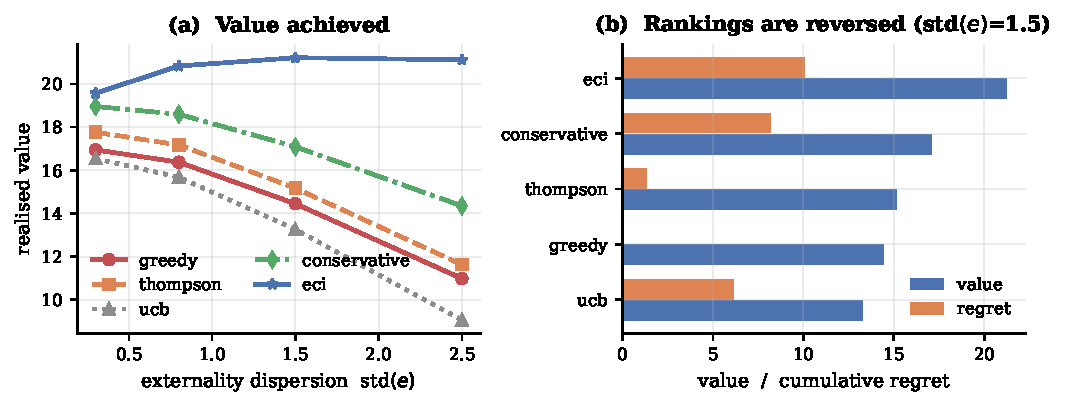
\includegraphics[width=\textwidth]{fig4_policies.pdf}
\caption{Policy comparison, $n=20$, $T=60$, 25 seeds. \textbf{(a)} Realised value
against externality dispersion. The corrected index dominates throughout, and its
margin widens as coupling strengthens. \texttt{conservative} uses no per-arm
knowledge at all and still beats every consumption-blind method. \textbf{(b)} Value
and cumulative regret side by side. The two orderings are close to reversed:
\texttt{greedy} records the lowest regret and near-lowest value; \texttt{eci}
records the highest regret and the highest value.}
\label{fig:policies}
\end{figure}

Thompson sampling is consistently \emph{worse} than greedy under known parameters.
Its exploration is not free here: sampling a suboptimal arm can destroy a
low-value, high-externality arm. At strong coupling the corrected index nearly
triples Thompson's realised value ($20.8$ vs.\ $7.2$). The mechanisms compose
rather than compete---TS handles uncertainty in $v$, ECI handles consumption---and
TS+ECI dominates both.

\section{Domains}
\label{sec:domains}

The model is not specific to agents. We instantiate it in four settings, each
supplying its own mapping to $(v,p,e,\delta)$ and each simulated rather than
merely described. Table~\ref{tab:domains} gives the mappings, and we state the
quality of fit honestly: two are close, one is a reasonable abstraction, and one is
partial.

\begin{table}[t]
\centering
\small
\caption{Domain instantiations. Each row is a running parameterisation, not an
illustration.}
\label{tab:domains}
\begin{tabular}{p{2.0cm}p{2.4cm}p{3.0cm}p{3.4cm}p{1.4cm}}
\toprule
domain & arm & destruction ($p$) & externality ($e$) & fit \\
\midrule
Agent tools & API-backed tool & call trips a rate limit, exhausts a quota, or
revokes a key & shared upstream infrastructure: burning one throttles the rest &
strong \\[2pt]
Adaptive therapy & dose level & dose exhausts the drug-sensitive cell population &
released resistant clone degrades all later treatment & strong \\[2pt]
Platform trial & treatment arm & arm dropped for futility on evidence the
allocation generated & reliance on shared control; removal degrades concurrency for
all comparisons & moderate \\[2pt]
Design space & process parameter setting & run consumes scarce material or yields
an out-of-spec batch & failure narrows the defensible filing envelope for all
settings & partial \\
\bottomrule
\end{tabular}
\end{table}

\paragraph{Adaptive therapy is the sharpest case.} Under maximum tolerated dose,
clinicians administer the highest tolerable dose, which is \emph{exactly} the greedy
policy. Higher dose intensity raises immediate tumour control $v$, but also raises
both the chance of exhausting the drug-sensitive population ($p$) and the damage
done when that happens ($e$), because the sensitive population was suppressing the
resistant clone. Since $v$, $p$ and $e$ rise together, $\kappa = pe$ is highly
dispersed---precisely the regime where Theorem~\ref{thm:char} says greedy fails. The
model therefore reproduces \emph{competitive release} from first principles: it
predicts that MTD is beaten by a dose-modulating policy, which is what adaptive
therapy trials find. We stress this is a reduced form; real tumour dynamics are a
population process, not additive burden from dead arms.

\paragraph{Results.} Figure~\ref{fig:domains} runs all four. In all four, greedy records cumulative regret of exactly $0.0000$ and is beaten---by
$30$--$49\%$ where $\kappa$ dispersion is largest. Thompson sampling,
which is consumption-blind, gains at most $7\%$ and in the agent domain is
\emph{worse} than greedy. The conservative policy, which uses no per-arm
externality knowledge whatsoever, matches or beats the fully-informed index in
three of the four tested domains---the practical form of Theorem~\ref{thm:floor}.

\begin{figure}[t]
\centering
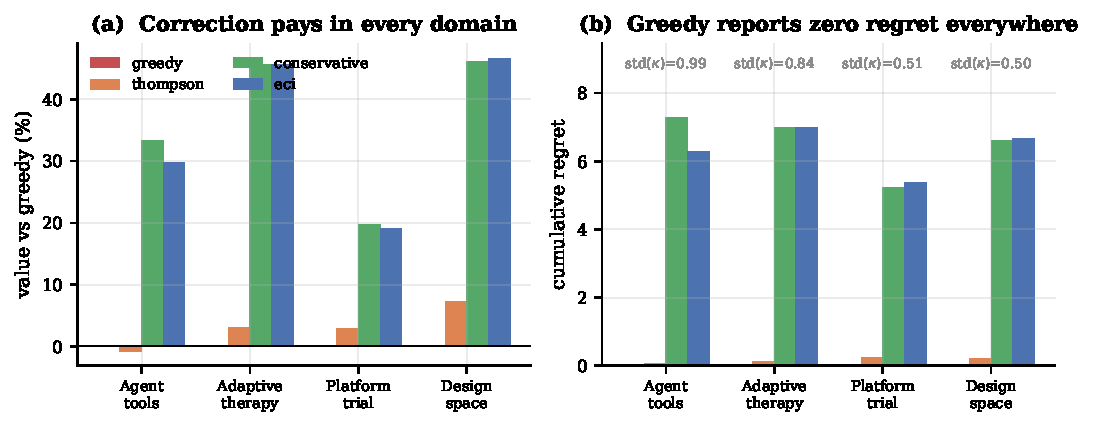
\includegraphics[width=\textwidth]{fig6_domains.pdf}
\caption{Four domains, 30 seeds each. \textbf{(a)} Value relative to greedy.
Correction pays in all four tested domains, most where $\kappa$ dispersion is
largest.
\textbf{(b)} Cumulative regret. Greedy sits at exactly zero in all four domains
while losing in all four. The consumption-blind baselines cluster near zero regret
with it; the policies that actually perform are the ones the metric penalises.}
\label{fig:domains}
\end{figure}

\subsection{Agent tool ecosystems in detail}

Figure~\ref{fig:trace} returns to the routing example of Section~1 and shows the
three quantities side by side over a single session. Panel (a) is what an
operations dashboard displays; panels (b) and (c) are what is actually happening.
The greedy router's regret trace is a flat line at zero for the entire session. Its
value per call steps downward three times, and its tool count falls to one. The
corrected router shows visible, non-zero regret throughout---and ends the session
delivering more value per call with more tools still alive.

\begin{figure}[t]
\centering
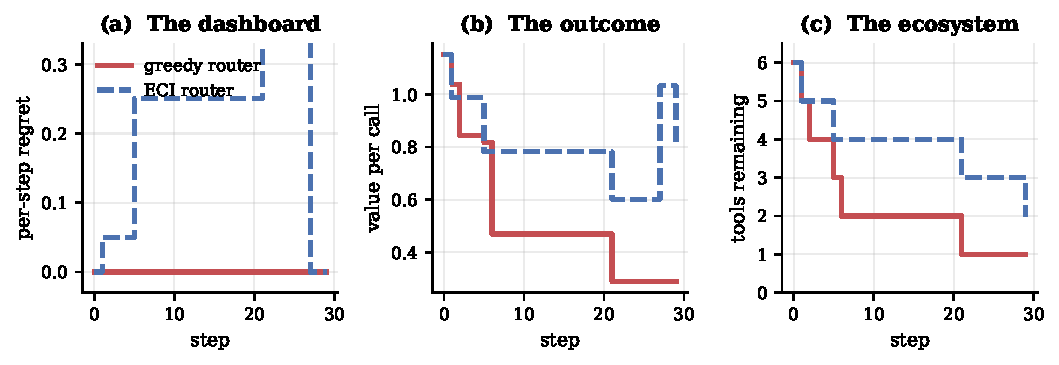
\includegraphics[width=\textwidth]{fig5_agent_trace.pdf}
\caption{A single routing session, identical seed and tool set. \textbf{(a)} The
metric: greedy's per-step regret is zero throughout, while the corrected router
accrues visible regret. \textbf{(b)} Value per call: the router with worse regret
delivers more. \textbf{(c)} Surviving tools: the router with worse regret preserves
more of the ecosystem. The visible regret in (a) is the \emph{price of
preservation}, and the standard metric records it as a defect.}
\label{fig:trace}
\end{figure}

This is the practical form of Theorem~\ref{thm:vacuity}. Nothing in panel (a)
would trigger an alert, a rollback, or a model review. The failure is invisible to
the instrument.

\section{Robustness to the coupling form}
\label{sec:robust}

The additive burden $B(S) = \delta\sum_{\text{dead}} e_i$ is a modelling choice, so
we test it against four alternatives under exact dynamic programming:
multiplicative (rewards scaled by $\prod(1-\delta e_i)$), saturating
($B_{\max}(1-e^{-\delta\sum e_i})$), networked (only graph-neighbours of the dead
arm are harmed), and concave ($\delta(\sum e_i)^{0.6}$).

\paragraph{Theorem~\ref{thm:vacuity} is robust to all five.} Greedy records regret
of exactly $0.0000000000$ under every coupling form while incurring positive value
loss under every one ($0.49$--$1.38$). This follows from the proof: zero regret is a
consequence of greedy's definition against the best-available benchmark, not of the
burden's functional form.

\paragraph{Theorem~\ref{thm:char} requires separability.} Here the picture is more
interesting. The characterisation holds exactly for additive, multiplicative and
networked coupling (gap $0.000000\%$ under constant $\kappa$), and fails slightly
for saturating ($0.098\%$) and concave ($0.674\%$). Measuring the marginal burden of
destroying one arm at different levels of accumulated damage identifies why: for
additive and multiplicative coupling that marginal burden is invariant
($0.15000$ at zero, three and six units of prior damage), whereas for saturating and
concave it falls as damage accumulates ($0.167 \to 0.107 \to 0.068$ and
$0.150 \to 0.055 \to 0.043$ respectively).

\begin{corollary}[Scope of Theorem~\ref{thm:char}]
The characterisation holds exactly when the burden is \emph{additively separable}
across destroyed arms---when an arm's contribution does not depend on what else has
already been destroyed. Under non-separable aggregation, constant $\kappa$ no longer
renders the burden term arm-independent.
\end{corollary}

This is a sharper statement than the original, not a weaker one: it names the
structural property the result requires. The degradation is also graceful---the
residual gap under non-separable coupling is $0.10\%$--$0.67\%$, against the
$6.6\%$--$12.2\%$ gap greedy incurs when $\kappa$ genuinely varies.

\section{Limitations}

Exact optimality results rest on dynamic programming at $n \le 8$;
larger-scale claims rest on rollout, and the coupling-robustness study of
Section~\ref{sec:robust} inherits the same ceiling. Theorem~\ref{thm:vacuity} is a statement about
the best-available-arm benchmark specifically---a forward-looking benchmark would
not be fooled, but it is also not what deployed systems measure, which is the point.
Theorem~\ref{thm:char}'s sufficiency proof relies on a coupling argument whose
formalisation under horizon truncation we verify exhaustively rather than prove in
full generality.

The domain instantiations vary in fidelity. The agent and adaptive-therapy mappings
are structurally faithful; the platform-trial mapping treats an inferential
externality (loss of concurrent control) as if it were a reward penalty, and mixes
patient benefit with information gain in a single scalar; the design-space mapping
omits the terminal-commitment layer that defines the real problem---a one-shot
declaration of design-space width that fixes the feasible set permanently. That
layer is an optimal-stopping problem on top of the bandit and is, in our view, the
most promising direction this work opens.

\section{Conclusion}

When actions consume the action set, regret is measured against an optimum the
learner has already degraded. A policy can hold regret at exactly zero while
driving value arbitrarily negative, and the parameter that would let it do better admits an
irreducible estimation error that worsens precisely as it becomes important, because
acquiring each observation destroys the resource being priced. The practical consequence is
direct: for irreversible actions, externality costs must be \emph{specified}, not
discovered. A crude uniform upper bound outperforms every learned estimator we
tested.

\paragraph{Code and reproducibility.} The library, all 27 experiments including the
falsified ones, and one regression test per theorem are released openly.
Every figure regenerates from the library and the exact-DP reference via a single
command, all random seeds are fixed and stated in code, and the test suite fails if
any theorem's numerical claim breaks.
\textbf{[Repository URL to be inserted before posting.]}

\begin{thebibliography}{9}
\bibitem{badanidiyuru2013} A.~Badanidiyuru, R.~Kleinberg, A.~Slivkins.
  Bandits with knapsacks. \emph{FOCS}, 2013.
\bibitem{chakrabarti2008} D.~Chakrabarti, R.~Kumar, F.~Radlinski, E.~Upfal.
  Mortal multi-armed bandits. \emph{NeurIPS}, 2008.
\bibitem{kleinberg2010} R.~Kleinberg, A.~Niculescu-Mizil, Y.~Sharma.
  Regret bounds for sleeping experts and bandits. \emph{Machine Learning}, 2010.
\bibitem{levine2017} N.~Levine, K.~Crammer, S.~Mannor.
  Rotting bandits. \emph{NeurIPS}, 2017.
\bibitem{seznec2019} J.~Seznec, A.~Locatelli, A.~Carpentier, A.~Lazaric,
  M.~Valko. Rotting bandits are no harder than stochastic ones.
  \emph{AISTATS}, 2019.
\bibitem{seznec2020} J.~Seznec, P.~Menard, A.~Lazaric, M.~Valko.
  A single algorithm for both restless and rested rotting bandits.
  \emph{AISTATS}, 2020.
\bibitem{shah2018} V.~Shah, R.~Johari, J.~Scheinkman.
  Bandit learning with positive externalities. \emph{NeurIPS}, 2018.
\end{thebibliography}

